%!TEX root = ../thesis.tex

\chapter{Conclusion}
\label{chp:conclusion}

Find an overview of this thesis as a whole in figure \ref{fig:overview}.
As a first step, the MINRV8 architecture inspired by the RISC-V architecture was defined and implemented in nuXmv in section \ref{sec:minrv8}.
In chapter \ref{chp:ifc}, we developed information flow semantics and three information flow properties forming an information flow control in spirit of the work of \citeauthor{Ferraiuolo17} \cite{Ferraiuolo17}.
The information flow semantics were used to augmented the model of the MINRV8 by information flow tracking.
In chapter \ref{chp:results} we introduced eight assumptions that, when implemented software running in machine-mode such as \glspl{os}, guarantee the absence of vulnerabilities covered by aforementioned information flow properties.
We evaluated our model, the properties and the assumptions by showing that taken together, they manage to detect both the cache poisoning \cite{Wojtczuk09} and the SYSRET vulnerability \cite{Dunlap19}.
Finally in chapter \ref{chp:discussion}, we discussed the limitations and the scope of our work and reflected whether our methodology is trustworthy.

\begin{figure}
    \centering
    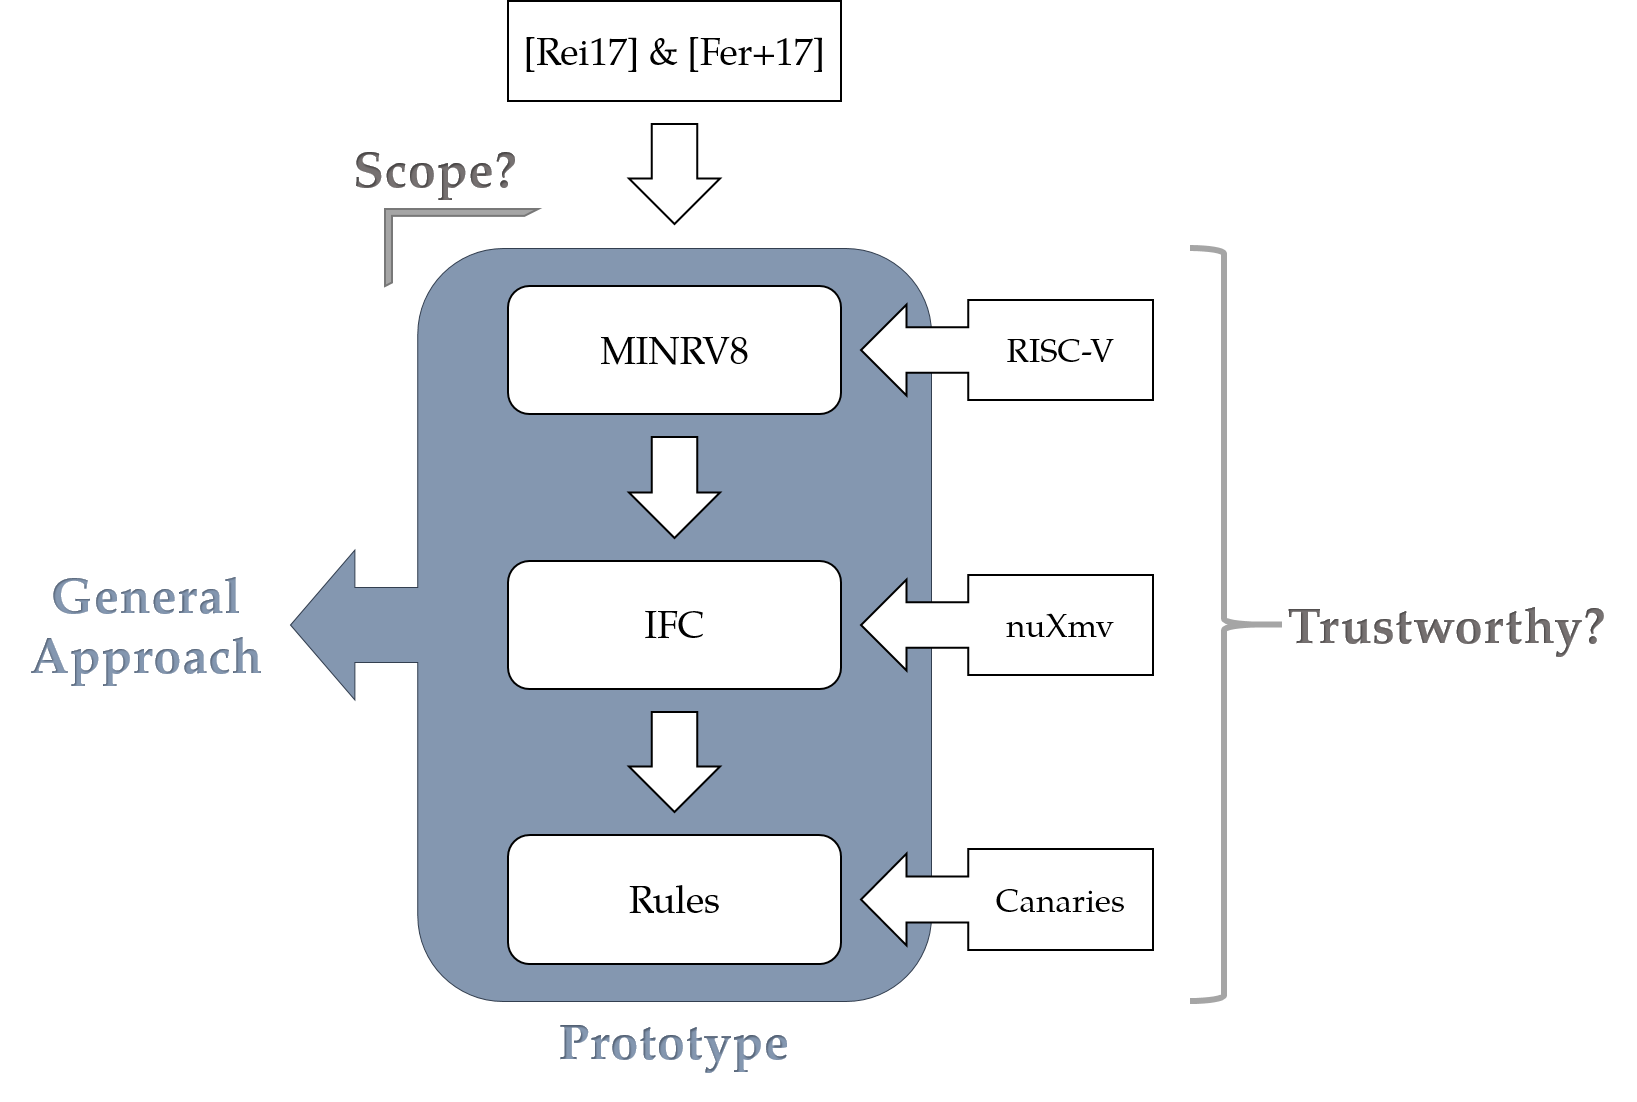
\includegraphics[width=\textwidth]{figures/thesis-overview.png}
    \caption{Thesis Overview}
    \label{fig:overview}
\end{figure}

In the introduction, we set three other goals: it was claimed that the approach presented as part of this thesis is \textit{viable}, i.e. feasible, realistic and generalizable, \textit{relevant}, i.e. it is able to detect issues, and \textit{supplemental}, i.e. it enhances on related work.

We were able to show the the implementation of the MINRV8 architecture models the property \enquote{assumptions $ \Leftrightarrow $ properties}.
This was put to a test by showing that said implementation does violate the properties as presented in section \ref{sec:ifc-properties} when it is exposed to the cache poisoning or SYSRET vulnerability.
In other words: it was shown that the three properties \smv{MEMORY_OP_INTEGRITY}, \smv{CSR_INTEGRITY} and \smv{NO_LEAK} cover at least vulnerabilities related to the cache poisoning or SYSRET vulnerability.
This marks the main result of this thesis and shows that this work is \textit{relevant}.
Furthermore, mitigations to these vulnerabilities can be verified using the same model.
It must be decided on a case by case basis whether a given violation of the information flow properties actually marks a vulnerability of the architecture leaving it with the need to be altered or marks a feature the risks of which must be controlled in software.
To achieve this, a novel approach of using model checking for verifying architectural specifications was used.
We discussed another case where model checking was applied to architectural specifications in \ref{sec:related-model-checking} \cite{BradfieldS16}.
However, this approach was flawed, did not use model checking to its full potential and implemented a very limited model
In \cite{BradfieldS16}, the properties only took one transition in the state spaces into consideration whereas in this work we proved properties touching traces of possibly infinite length.
Additionally, in \cite{BradfieldS16}, the model only comprised instructions related to mode-transitioning whereas here, we implemented a more or less complete set of basic \gls{risc} instructions.
This, taken together with the discussion of other related work in chapter \ref{chp:related-work} shows that this work is \textit{supplemental}.

What is left to show is that this work is \textit{viable}.
All proofs were run on a laptop equipped with an Intel Core i7-7500U CPU with 8GB of RAM.
It is safe to say, that these are very moderate hardware requirements.
Proofs were conducted per property.
None of these proofs took more than 60s.
While we can give no clear count of working hours spent on this thesis, all of it was developed and written by a single person in no more than eight months.
During this time, this person did not solely work on this thesis.
In a non-research scenario one can assume that development would be more straight forward since it would not include the definition of an architecture.
Due to the exponential blow-up of binary encoded state spaces, there are no guarantees that this approach scales well to realistic and complete architectures.
However, there are two reasons which make seem likely that this approach does indeed scale.
Firstly, the proofs here were ran on a small machine and didn't take much time.
\todo{Strenghtened by related work, i.e. IFT in OS track by one label only}
Secondly, in section \ref{sec:discuss-observations} it was discussed that bit-wise tracking of information flow might be dropped, i.e. there is room for performance improvements.
All of this gives good reasons to believe that our approach is indeed \textit{viable} and could be applied to other architectures with reasonable effort.

\todo[inline]{Bridge}

In section \ref{sec:verify-spec} four design goals were discussed that were initially introduced in \cite{Reid17}.
These were defined to apply to high level properties for specifications and list as follows:
\begin{displaycquote}[pp.88:2-3]{Reid17}
    The central design challenge we face is to create a set of properties that:
    \begin{itemize}
        \item express the major guarantees that programmers depend on;
        \item are concise so that architects can easily review and remember the entire set of properties;
        \item are stable so that architectural extensions don't invalidate large numbers of rules;
        \item and that describe the architecture differently from existing specification to reduce the risk of common-mode failure.
    \end{itemize}
\end{displaycquote}

These objectives are met by our work:
\begin{itemize}
    \item The assumptions guarantee programmers of \glspl{os} and compilers that programs adhering to these do not violate basic information flow properties.
    \item Both assumptions and properties are small in number and short and can be expressed in intuitive natural language, hence concise.
    \item The properties itself are completely architecture independent and as such stable.
    The assumptions are architecture dependent and rely on both instructions available and concrete semantics of these instructions.
    However, we feel subjectively that only basic mechanics are used and predict that the assumptions in a practical environment of an architecture subject to change should be relatively stable as well.
    \item The premise of information flow tracking on instruction level is to describe the architecture from a different point of view.
    It is therefore obvious that there is very little risk of common-mode failure.
\end{itemize}

Finally, we give an outlook on future work:
\begin{description}
    \item[Executable memory] First and foremost, the model could be enhanced by a model of executable memory to more closely resemble modern architectures.
    This was discussed extensively in section \ref{sec:discuss-arch}.
    \item[MMU] In light of \cite{KhakpourSD13} a model of an \gls{mmu} could be implemented to make use of information flow tracking on user-mode level.
    This was discussed in chapter \ref{chp:related-work}.
    \item[Machine-generated model] The model of the architecture that was implemented by hand in this thesis could be generated from existing machine-readable architectural specifications.
    For example, there are machine-readable versions of the ARM architecture; both \cite{Reid17,Fox02} either used or developed machine-readable specifications that might be used for this endeavor.
    For RISC-V, there also is a formal specification available \cite{RiscvSpecFormal}.
    Not implementing the model by hand would \begin{enumerate*}[label=\alph*)]
        \item possibly enhance the trust in the model itself, depending on the trust in the source and the translation procedure, and
        \item make the approach even more viable and stable towards architectural changes.
    \end{enumerate*}
    \item[Complete model] An obvious improvement of this work would be to enhance it by more instructions and use a bigger word-size.
    This would bring the model closer to real-world architectures but might also introduce performance issues.
    \item[Verification of assumptions] Finally, it could be investigated whether the assumptions introduced in context of the verification process serve as practical and sensible target of verification for compilers and/or \glspl{os}.
    It could be investigated whether code generated from compilers or \glspl{os} itself adheres to these assumptions.
    Applying the assumptions to the next level of abstraction in modern computing might lead to more easy and mainstream usage of formal verification in programming.
    Since these properties are stable for a given architecture, there could be off the shelf tools verifying programs for high-level correctness removing the need to tailor verification efforts per system to be verified.
\end{description}

\todo[inline]{Final summary}
